\section{Basic Theory}

When dealing with systems with a lot of content it can cause information overload for its users.
Information overload can be minimized through recommender systems.
There are broadly speaking two approaches to recommender systems which are content-based filtering and collaborative filtering.
Content-based filtering tries to recommend items that are similar to items that the user has liked before.
Collaborative filtering on the other hand uses both relationship between users and the inter dependencies among items to provide recommendations \cite{Matrix-factorization-techniques}.
This means that collaborative filtering recommends an item to a user based on a similar user.

Collaborative filtering does often only utilize users and their rated items, but it can still recommend items that are difficult to profile using content-based filtering \cite{Matrix-factorization-techniques}.
However, collaborative filtering suffers from the cold start problem which means that it does not deal well with new users that have not rated any items.
Throughout this section we look at some collaborative filtering methods, as it is more related to the methods that we have investigated in this paper.
We also explain some theory behind Neural Networks and Graph Convolutional Network.

\subsection{Matrix factorization}\label{bsc::MF}
The data concerning users and items can be represented as a matrix where each row represents a user and each column an item.
The entries in the matrix will then be the explicit feedback given for that item by the user if there is any.
This will for larger datasets be a sparse matrix as all users usually will not interact with most items.
Matrix factorization can then be used to infer user preference for the items not rated by the user by using implicit feedback which can be purchase history, browsing history, mouse movement or any behavioral patterns that the user has.
We can estimate if a user is going to like an item by analyzing the behavior of the users \cite{Matrix-factorization-techniques}.
We start out with a matrix $A = N x M$ where N is the number of users and M is the number of items.
The implicit feedback is used to learn the latent features of the items and the users liking of those latent features.
This is done by mapping users and items to a joint latent factor space of dimensionality $f$.
The items will then be associated with a vector $q_i \: \epsilon \: \mathbb{R}_f$ and the user will be associated with a vector $p_u \: \epsilon \: \mathbb{R}_f$.
The matrix $q$ has the dimensions $k x m$ where k is the number of latent features and m is the number of items.
Matrix $p$ has the dimensions $n x k$ where n is the number of users and k is the number of latent features.
For each item $i$ the corresponding entry in $q$ will measure the extent in which the item possesses the feature and for each user u the corresponding entry $p_u$ in $p$ will measure their liking to each feature.
By then calculating the dot product $q^T \cdot p$ the resulting matrix will capture an estimate of what each user would rate each item.
The main challenge of using the matrix factorization model is finding a good algorithm for computing the mapping of each item to the factor vectors $q_i$ and $p_u$.
After the factor vectors are computed the task of estimating the rating a user will give an item is easy through the following equation $r_{ui} = q_i^T p_u$ where $r_{ui}$ is the resulting ratings matrix.

\subsection{Factorization machines}
Factorization machines(FM) are a general-purpose supervised learning algorithm and were originally introduced by Steffen Rendle \cite{factorization_machines}.
The main advantage of using FM's is that they perform well with large and sparse datasets, and have a linear complexity.
When dealing with very sparse datasets where there are many users and items with few interactions, it can be difficult to predict future interactions because there is not enough data to do so.
This is the problem that FM's solve.
FM's are able to do this well because they break the independence of the parameters by factorizing them.
This means that they can utilize the data of one interaction to estimate the data for another interaction.
Unlike classic matrix factorization models which represents the interactions as a matrix with users and items the FM model represents user-item interactions as tuples of real-valued feature vectors and numeric target variables.
If we take the yelp data that we have used in \autoref{equal-data} as an example.
In this data set we have set of users U, items I, categories C and price levels P.
\begin{itemize}
    \item $U = {1, 2}$
    \item $I = {1, 2 ,3}$
    \item $C = {1, 2}$
    \item $P = {1, 2}$
\end{itemize}
These are the categorical variables in the data set.
The interactions in this dataset would then be represented as seen in \autoref{fig:FM-example} where each interaction is a row in the table which in the FM model is considered a feature vector.
The last column contains the target variables for the corresponding row.
The target variable is the feature that the model wants to learn from the other features.
This means that it will try to learn what the relationship is between the combination of features in the feature vector and the value of the target variable.
This is how supervised machine learning algorithms generally learn.
\begin{figure}
    \centering
    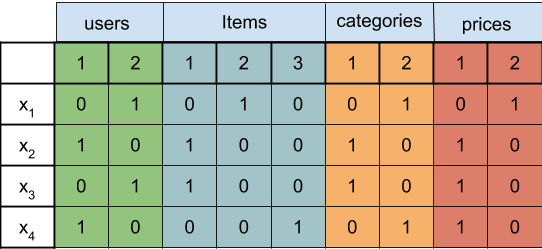
\includegraphics[scale=0.35]{figures/FM-example.png}
    \caption{Dataformat used in FM's}
    \label{fig:FM-example}
\end{figure}
The goal of the FM model is to estimate a function $\hat{y}$ from a feature vector $x_i$ to a target domain.
It does this by using factorized parametrization to capture feature interactions.

The equation for the model looks like this:
\[ \hat{y}(x) := w_0 + \sum_{i=1}^{n} w_ix_i + \sum_{i=1}^{n}\sum_{j=i+1}^{n} \big \langle v_i,v_j \big \rangle x_ix_j, \]
where the parameters that have to be estimated are:
\[ w_0 \epsilon \mathbb{R}, \qquad \mathbf{w} \epsilon \mathbb{R}^n, \qquad  \mathbf{V}\epsilon \mathbb{R}^{n \times k} \]
and $\big \langle v_i,v_j \big \rangle$ is the dot product of two vectors of size k:
\[ \big \langle v_i,v_j \big \rangle := \sum_{f=1}^{k} v_{i,f} \cdot v_{j,f}\]

\begin{itemize}
    \item $w_0$ which is the global bias
    \item $w_i \epsilon \mathbb{R}^n$ are the weights for feature vector $x_i$
    \item $V \epsilon \mathbb{R}^{nxk}$ is the weight matrix for feature vector combination $v_iv_j$
\end{itemize}
A row $v_i$ within V describes the i-th variable with k factors.
k is a hyperparameter that defines the dimensionality of the factorization.
By doing this the FM models each interaction by factorizing it which allows it to estimate parameters of high-order interactions under sparsity.

\subsection{Neural Networks}
Neural networks are a multi-layered collection of nodes which have an input layer, hidden layers, and an output layer \cite{AI-book}.
The input of each node is the output of all nodes in the previous layer.
Each of these connections in the network has an individual weight associated with it.
To get the value of a node not in the input layer, the output of all the nodes in the previous layer are added together with each individual weight along the connection that it travels.
All these weighted values are then fed to an aggregation function which result is given to an activation function.
The activation function is usually the Sigmoid, Sign, or Relu function.
\\
Neural networks can have any number of nodes in the input layer, hidden layers, and output layer and they do not need to be the same amount.
Furthermore, it can have any number of hidden layers.
\\
Neural networks have had considerable success in low-level reasoning where lots of training data are available.
They learn by giving the input layer values and then have the network compute an output value.
The output value is then compared to the real value of the inputs and based on the margin of error we go backwards through the network adjusting each weight.
This is called back propagation.
After doing this enough times or when the margin of error is lower than a predefined value the network is considered trained and can be tested on new data or be applied to a real-world scenario.

\subsubsection{Bayesian Personalized Ranking}\label{subsubsec:BPR}
Bayesian Personalized Ranking(BPR) is an approach to modeling personalized ranking \cite{BPR}.
This is done through a pairwise approach where we calculate the probability that a user $u$ prefers item $i$ over item $j$.
It calculates the probability value of a user preferring $i$ over $j$ for every item pair and then maximizes the log-likelihood of all the observed pairs.
In NGCF, LightGCN and Price-Aware Recommendation they use BPR as their loss function.
This is done by taking the objective function of BPR $x_{uij}$ and negating it.
The equation for the loss function will then look like this:
\[E(x_{uij}) = ln(1+e^{-x_{uij}})\]

\subsubsection{Adam optimization algorithm}\label{subsubsec:Adam}
The way that Adam differs from the classical Stochastic gradient descent algorithm is that instead of having a single learning rate for all weights, it has a learning rate that is maintained for each network weight\cite{Adam}.
This learning rate is then separately adapted during the learning process.
The algorithm combines the advantages of two stochastic gradient descent algorithms Adaptive Gradient Algorithm (AdaGrad) and Root Mean Square Propagation (RMSProp).
Adam calculates an exponential moving average of the gradient and the squared gradient.
It then has two parameters $\beta_1$ and $\beta_2$ that control the decay of these moving averages.
The Adam optimization algorithm is implemented and can be used freely in both PyTorch and Tensorflow.
It is also an efficient algorithm that has little memory requirements.
The efficiency, availability and performance of the algorithm makes it a good candidate for many machine learning problems.
The main papers that we investigated LightGCN \cite{lightgcn} and Price-aware Recommendation\cite{Priceaware}, both use Adam as their optimization algorithm.


\subsection{Graph Convolutional Network}
Graph Convolutional Network (GCN) is a neural network architecture that operates on graphs.
Given a graph $G = (V,E)$ a GCN takes an adjacency matrix $A$ as input with the size of $N x N$ that represents graph $G$ and a feature matrix $N x F^0$, where $N$ is the total amount of nodes and $F^0$ is the total amount of input features for each node.
A hidden layer in a GCN can be defined as $H^i = f(H^{i-1}, A)$ where $i$ indicates the layer, $H^0$ is the previously mentioned $N x F^0$ feature matrix and $f$ is a propagation function \cite{Deep-Learning-on-Graphs-with-GCN}.
There are many different types of propagation functions.
A simple example could be $f(H^i, A) = \sigma(AH^iW^i) = H^{i+1}$ where $W^i$ is the weight matrix at layer $i$ and $\sigma$ is a non-linear activation function \cite{Deep-Learning-on-Graphs-with-GCN}.
The intuition behind this propagation function is that the future representation of each node is calculated based on its neighbors nodes.
Because of this, each time $i$ is increased, a node's new value is therefore affected not only by its neighbors but its neighbors' neighbors and so on.
An issue with this propagation function could be that the value of each node now is a sum of each of its neighbors, and therefore loses its own value.
This could be solved by replacing $A$ with $\hat{A} = A + I$ where $I$ is the identity matrix.
Doing this the node considers itself a neighbor.
